%! TEX PROGRAM = pdflatex
\documentclass[a4paper]{article}

\usepackage[utf8]{inputenc}
\usepackage{microtype, listings, amsmath, amssymb, csquotes}
\allowdisplaybreaks
\usepackage{tikz}
\usepackage{pgfplots}
\usepackage{subcaption}
\usepackage{xparse}
\usepackage{graphicx}
\usepackage{bm}
%\usepackage{subfig}

\usepackage{alphalph}
\usepackage[hidelinks]{hyperref}
\usepackage{cleveref}
\usepackage[margin=1in]{geometry}

\usepackage[style=numeric,sorting=none]{biblatex}
\addbibresource{main.bib}

\hypersetup{
    colorlinks=true,
    linkcolor=red,
    citecolor=green,
    filecolor=magenta,
    urlcolor=cyan
}


\newenvironment{psmallmatrix}
  {\left(\begin{smallmatrix}}
  {\end{smallmatrix}\right)}

\newcommand{\wrt}{w.r.t.}
\DeclareMathOperator*{\argmax}{arg\,max}
\DeclareMathOperator*{\argmin}{arg\,min}

%was node [circle,draw=black,inner sep=0pt,minimum size={width("AAA")}] {\AlphAlph{\x}\AlphAlph{\y}};}}
% was [square,draw=black]
\providecommand{\toroid}[1]{
    \draw[shift={(-0.5,0.5)}] (1,-1) grid (#1+1,-#1-1);
        \foreach \x in {1,...,#1} {
            \foreach \y in {1,...,#1} {
                \node at (\x,-\y) {\AlphAlph{\y}\AlphAlph{\x}};}}
}
\providecommand{\superToroid}[4]{
    \IfBooleanTF#1{\providecommand{\shading}{white}}{\providecommand{\shading}{gray}}
    \draw[shift={(-0.5,0.5)}] (1,-1) grid (#2+1,-#2-1);
        \foreach \x in {1,...,#2} {
            \foreach \y in {1,...,#2} {
        \pgfmathtruncatemacro{\xpos}{(\x-1)*#2+(\y-1)}
        \pgfmathtruncatemacro{\ypos}{((#4-1)*#2+(#3-1))}
        \ifnum\xpos<\ypos
        \providecommand{\param}{white}
        \else
        \providecommand{\param}{\shading}
        \fi
\node[square,draw=black,fill=\param] at (\x,-\y)[align=center] {\AlphAlph{#3}\AlphAlph{#4}\\ \AlphAlph{\y}\AlphAlph{\x}};}}
}
\providecommand{\toroidWarp}[1]{
    \scalebox{0.8}{
    \begin{tikzpicture}
        \toroid{#1}
        \foreach \x in {1,...,#1} {
            \node at (\x,0) {\AlphAlph{#1}\AlphAlph{\x}};
            \node at (\x,-#1-1) {\AlphAlph{#1}\AlphAlph{\x}};
        }
        \foreach \y in {1,...,#1} {
            \node at (0,-\y) {\AlphAlph{\y}\AlphAlph{#1}};
            \node at (#1+1,-\y) {\AlphAlph{\y}\AlphAlph{1}};
        }
    \end{tikzpicture}
}}

\providecommand{\toroidAxes}[4]{
    \superToroid{#1}{#2}{#3}{#4}
        \foreach \x in {1,...,#2} {
            \node at (\x,0) {\AlphAlph{\x}};
        }
        \foreach \y in {1,...,#2} {
            \node at (0,-\y) {\AlphAlph{\y}};
        }
}

\NewDocumentCommand{\nestedToroid}{sm}{
    \scalebox{0.8}{
    \begin{tikzpicture}[scale=#2+1,square/.style={rectangle,inner sep=0pt,minimum size=1cm}]
        \begin{scope}[scale=1]
            \draw[shift={(-0.5,0.5)}] (1,-1) grid (#2+1,-#2-1);
            \foreach \x in {1,...,#2} {
                \node at (\x,-0.25) {\AlphAlph{\x}};
            }
            \foreach \y in {1,...,#2} {
                \node at (0.25,-\y) {\AlphAlph{\y}};
            }
            \foreach \xa in {1,...,#2} {
                \foreach \ya in {1,...,#2} {
                    \begin{scope}[shift={({\xa-0.5+1/(#2+1)^2},{-\ya+0.5-1/(#2+1)^2})},scale={1/(#2+1)}]
                        \toroidAxes{#1}{#2}{\xa}{\ya}
                    \end{scope}
                }
            }
        \end{scope}
    \end{tikzpicture}
    }
}
%a
\NewDocumentCommand{\twodcomparison}{sm}{
    \IfBooleanTF#1{\providecommand{\shading}{white}}{\providecommand{\shading}{gray}}
    \scalebox{0.8}{
\begin{tikzpicture}
    \begin{scope}[square/.style={rectangle,inner sep=0pt,minimum size=1cm}]
        %\draw[shift={(-0.5,0.5)}] (0,0) grid ({(#2^2)},{-(#2^2)});
        \foreach \x in {1,...,#2} {
            \foreach \xa in {1,...,#2} {
                \node at ({(\x-1)*#2+(\xa-1)},1) {\AlphAlph{\x}\AlphAlph{\xa}};
        }}
        \foreach \y in {1,...,#2} {
            \foreach \ya in {1,...,#2} {
                \node at (-1,{-((\y-1)*#2+(\ya-1))}) {\AlphAlph{\y}\AlphAlph{\ya}};
        }}
        \foreach \xa in {1,...,#2} {
            \foreach \ya in {1,...,#2} {
            \foreach \xb in {1,...,#2} {
                \foreach \yb in {1,...,#2} {
                \pgfmathtruncatemacro{\xpos}{(\xa-1)*#2+(\ya-1)}
                \pgfmathtruncatemacro{\ypos}{((\xb-1)*#2+(\yb-1))}
                %\pgfmathtruncatemacro\xpos{}
                %\pgfmathtruncatemacro\ypos{}
        \ifnum\xpos<\ypos
        \providecommand{\param}{white}
        \else
        \providecommand{\param}{\shading}
        \fi
\node[square,draw=black,fill=\param] at (\xpos,-\ypos)[align=center] {\AlphAlph{\xa}\AlphAlph{\ya}\\ \AlphAlph{\xb}\AlphAlph{\yb}};}}
            }
        }
    \end{scope}

\end{tikzpicture}
}}

\title{Toroidal Grid Optimization via Gradient Descent}
\author{Jason Ken A}

\begin{document}
\maketitle
\tableofcontents

\section{Introduction}%
\label{sec:introduction}

Gradient descent is an iterative algorithm to optimize (to maximize or minimize) a continuous function. It does so by shifting the value of the paramaters in the direction of its gradient with respect to (\wrt{}) the function. In the context of minimization, it is defined as follows
\begin{align*}
         \theta'=\theta-\alpha \frac{d}{d\theta}L(\theta)
\end{align*}
where $\theta$ is the paramater to optimize with the goal of minimizing the value of the function $L$. $\alpha$ is a scaling factor representing how far the paramater should shift. This equation can be generalized to optimize many paramaters by utilizing partial derivatives instead. Anyhow, it is obvious why a continuous function is required: gradients are only defined with continuous functions.

The primary goal of this essay is to test whether a discrete loss function and its corresponding discrete paramaters can be generalized to a continuous loss function and continuous paramaters, with the purpose of finding optimum discrete variables. What better demonstration than its application on a difficult challenge? So, I chose to address this problem within the context of a programming contest called ``Reversing Nearness'' held by Al Zimmermann, which traditionally, had been approached with algorithms that do not utilize gradients, such as hill climbing (which modifies each paramater sequentially and keeps changes that optimize the function) and simulated annealing (which is essentially probabilistic hill climbing)\footnote{both of which are beyond the scope of this essay}. But I wanted to do it with gradients! Because what else would my calculus classes be for.

The objective of Al Zimmermann's programming contest, is to rearrange discrete tokens within a discrete grid, to minimize the the a loss function which depends on the distances between these tokens on a toroidal surface. The intricacies of this problem are explained within the essay.

Hence, my research question: \emph{Is gradient descent a viable approach for toroidal grid optimization?}

There are many techniques used within this essay to accomplish this goal. Among them are
\begin{enumerate}
  \item Generalization of Euclidean distances to accomodate toroidal surfaces
  \item Matric permutations to remove duplicate entries
  \item ``Superposition'' to model discrete tokens being within multiple positions, with their respective ``probabilities''\footnote{Probabilities here does not refer to the chance of a random event occuring, but rather the ``confidence'' in which a token is in its position, or the extent in which the position affects the loss function}
  \item Enforcement of probabilities (that they should sum to one), using the Sinkhorn-Knopp algorithm\cite{sinkhorn1967concerning}
  \item Use of Jacobian matrices for gradient descent
\end{enumerate}

\section{Problem Statement}%
\label{sec:problem_statement}

\subsection{Toroidal Grid}%
\label{sub:toroidal_grid}

As per AZsPCs\cite{zimmermann} specifications, the initial toroidal grid $O$ is defined as an $N\times N$ grid of unique tokens which ``wrap around'' the edges. A token is of the form $\bm{IJ}$, where $\bm{I}$ and $\bm{J}$ are alphabetic representations of the indices of the rows and columns respectively, of a token, \emph{within $O$},\footnote{This is important because after rearranging the tokens, the identity of the token depends on its position within $O$, and not the rearranged position} e.g., $AC$ corresponds to the token in row 1, column 3 of $O$, $DF$ corresponds to the row 4, column 6 of $O$, etc. \autoref{fig:toroidExample} shows $O$ for $N=4$. Tokens outside of the square grid represent tokens ``wrapping around'' the edges, resembling a toroidal surface as shown in \autoref{fig:wiki_toroid}.
\begin{figure}[htpb]
    \begin{subfigure}[t]{0.5\textwidth}
    \begin{center}
        \raisebox{0.4cm}{
        \includegraphics[width=0.7\textwidth]{images/Simple_Torus.pdf}}
    \caption{A Simple Toroid by Yassine Mrabet\cite{wiki_toroid}}
    \label{fig:wiki_toroid}
    \end{center}
    \end{subfigure}
    ~
    \begin{subfigure}[t]{0.5\textwidth}
    \begin{center}
    \toroidWarp{4}
    \caption{A $4\times 4$ \emph{intial} toroidal grid}%
    \label{fig:toroidExample}
    \end{center}
    \end{subfigure}
    \caption{Representations of a toroidal grid}
\end{figure}

\subsection{Evaluation Function}%
\label{sub:evaluation_function}

The goal of the challenge is to rearrange the tokens within $O$ to form a new grid $X$ that minimizes a loss function computed with the following procedure:
\begin{enumerate}
    \item For each unique pair of tokens (e.g., $[AA,BA]$ is equivalent to $[BA,AA]$, so $[BA,AA]$ is omitted), calculate the squared distance between them in $X$,
    \item Multiply each of these by the squared distance between the pair of tokens within $O$,
    \item Sum all of these products,
    \item Subtract a lower-bound corresponding to the value of $N$ (\autoref{sec:lower_bound_constants})
\end{enumerate}

\subsection{Distance Metric}%
\label{sub:distance_metric}
To evaluate the loss function, a distance metric between two tokens must be established, which necessitates a coordinate system. Here, \emph{the coordinate of a token is defined as the indices of the token within $X$} i.e., any token within row 5, column 3 of $X$, has coordinates $(5,3)$. Note that within $O$, coordinates, indices, and token representations are all equivalent.

 Let two two-dimensional coordinates be $s_1=(x_1,y_1)$ and $s_2=(x_2,y_2)$. The Euclidean distance $d_{euclid}$ is defined as,%
\begin{align}
    \label{eq:euclid}
    d_{euclid}(s_1,s_2)=\sqrt{(x_2-x_1)^2+(y_2-y_1)^2}=\sqrt{(\Delta_{euclid} x)^2+(\Delta_{euclid} y)^2}
\end{align}

On a toroidal surface however, $\Delta x$ and $\Delta y$ can each have 2 possible values. A one-dimensional toroidal surface of length $N$ is illustrated in \autoref{fig:2distanceexample}. The corresponding possible values for $\Delta x$ are as follows,%
\begin{align}
    \Delta_1(x)&=x_2-x_1\nonumber\\
    \Delta_2(x)&=(x_1-0)+(N-x_2)=x_1+N-x_2
    \label{eq:naiveToroidDistance}
\end{align}

\begin{figure}[htpb]
    \centering
    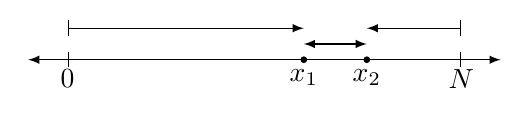
\begin{tikzpicture}
        \draw[latex-latex] (-3,0) -- (3,0);
        \draw[|-|] (-2.5,0) node[below] {$0$} -- (2.5,0) node[below] {$N$};
        %\draw[|-|] (-2.5,-0.5) -- node[below] {$N$} (2.5,-0.5);
        \filldraw (0.5,0) circle (1pt) node[below] {$x_1$};
        \filldraw (1.3,0) circle (1pt) node[below] {$x_2$};
        \draw[latex-latex] (0.5,0.2) -- (1.3,0.2);
        \draw[latex-|] (1.3,0.4) -- (2.5,0.4);
        \draw[|-latex] (-2.5,0.4) -- (0.5,0.4);
    \end{tikzpicture}
    \caption{A one-dimensional diagram of toroidal distance, with the two arrows representing two possible distances}%
    \label{fig:2distanceexample}
\end{figure}

To obtain a general equation that works when $x_1>x_2$:%
\begin{align}
    \Delta_1(x)&=\lvert x_2-x_1 \rvert\nonumber\\
    \Delta_2(x)&=\min{(x_1,x_2)}+N-\max{(x_1,x_2)}
    %\label{eq:absoluteToroidDistance}
\end{align}
where $\lvert a\rvert$ is the absolute value of $a$, $\min{(a,b)}$ and $\max{(a,b)}$ are defined as the minimum and maximum between the values of $a$ and $b$ respectively, that is,%
\begin{align}
        \min{(a,b)}=
        \begin{cases}
            a,&\text{if $a\leq b$}\\
            b,&\text{if $a>b$}
        \end{cases}\qquad
        \max{(a,b)}=
        \begin{cases}
            a,&\text{if $a\geq b$}\\
            b,&\text{if $a<b$}
        \end{cases}
\end{align}
$\min$ and $\max$ are used to determine the  ``left-most'' and the ``right-most'' coordinates.

One-dimensional toroidal distance is then defined as%
\begin{align}
    \Delta x=\min{(\Delta_1(x),\Delta_2(x))}
\end{align}

And in two dimensions, the toroidal distance and squared toroidal distance are%
\begin{align}
    d(s_1,s_2)&=\sqrt{(\Delta x)^2+(\Delta y)^2}\nonumber\\
    d^2(s_1,s_2)&=(\Delta x)^2+(\Delta y)^2
\end{align}
From now on, \emph{distance} refers to $d^2$.

For example, the distance between $s_1=(1,4),s_2=(2,1)$ and $N=5$ is calculated as follows:%
\begin{align}
    \Delta_1(x)&=\lvert 2-1\rvert=1\nonumber\\
    \Delta_2(x)&=\min{(1,2)}+5-\max{(1,2)}=1+5-2=4\nonumber\\
    \Delta_1(y)&=\lvert 1-4\rvert=3\nonumber\\
    \Delta_2(y)&=\min{(4,1)}+5-\max{(4,1)}=1+5-4=2\nonumber\\
    \Delta(x)&=\min{(1,4)}=1\nonumber\\
    \Delta(y)&=\min{(3,2)}=2\nonumber\\
    d^2(s_1,s_2)&=1^2+2^2=5
\end{align}

\subsection{Token Comparisons}%
\label{sub:token_comparisons}
\begin{figure}[htpb]
    \centering
    \begin{subfigure}[t]{0.5\textwidth}
    \begin{center}
    \nestedToroid{2}
    \end{center}
    \caption{}
    \label{fig:4dcomparison}
    \end{subfigure}%
    ~
    \begin{subfigure}[t]{0.5\textwidth}
    \begin{center}
    \twodcomparison{2}
    \end{center}
    \caption{}
    \label{fig:2dcomparison}
    \end{subfigure}

    \caption{Tensors $C(X)$ in the forms $C(X)_{i,j,k,l}$ and $C(X)_{m,n}$ respectively, representing comparison grids of an $N=2$ toroidal grid, where every element represents the distance between tokens $\bm{IJ}$ and $\bm{KL}$ within $X$. Shaded cells denote unique comparisons.}%
    \label{fig:comparisonGrids}
\end{figure}

In order to compute distances between all possible pairs, a corresponding representation is required, i.e., a 4-dimensional matrix (or tensor) with elements being distances between \emph{source} tokens (first 2 dimensions) and \emph{target} tokens (next 2 dimensions). An example of the structure of the comparison for an $N=2$ grid is shown in \autoref{fig:4dcomparison}.

\begin{figure}[htpb]
    \centering
    \flatten{3}
    \caption{Matrix-flattening}%
    \label{fig:matrix_flattening}
\end{figure}
The dimensionality of the grid can be reduced from a tensor into a matrix, to reduce complexity (e.g., number of $\Sigma$s in \ref{sub:loss_function_as_matrix_multiplications}) by applying the matrix-flattening scheme in \autoref{fig:matrix_flattening} twice, on the source and target dimensions, reducing $C(X)$ from $N\times N\times N\times N$ to $N^2\times N^2$. Elements within the 4-dimensional tensor are of form $C(X)_{i,j,k,l}$, whereas the 2-dimensional elements are of form $C(X)_{m,n}$. To do this conversion,%
\begin{align}
    m=(i-1)\times N+j &\implies m\div N=i-1 \text{ remainder } j\nonumber\\
    n=(k-1)\times N+l &\implies n\div N=j-1 \text{ remainder } l
    \label{eq:flattening_scheme}
\end{align}
\autoref{eq:flattening_scheme} can be understood by realizing that $A_{2,3}$ (\autoref{fig:matrix_flattening}) is offset by $(2-1)$ groups of 3 and an additional 3 after flattening.

Note that both $C(X)_{i,j,k,l}$ and $C(X)_{m,n}$ represent the distance between tokens $\bm{IJ}$ and $\bm{KL}$ within $X$ as defined within \autoref{sub:distance_metric}, the difference lies only within their dimensionality. The two-dimensional representation of \autoref{fig:4dcomparison} is shown in \autoref{fig:2dcomparison}.

From now on, let $C(X)$ refer to the two dimensional comparison grid. Examples are shown in \autoref{fig:comparisonExample}.

\begin{figure}[htpb]
    \begin{subfigure}[b]{0.5\textwidth}
    \begin{center}
\drawGrid{2}{{AA,AB,BA,BB}}
    \end{center}
    \caption{$O$}
    \end{subfigure}%
    \begin{subfigure}[b]{0.5\textwidth}
    \begin{center}
        \begin{align*}
            \begin{blockarray}{ccccc}
            &AA & AB & BA & BB \\
            \begin{block}{c[cccc]}
                AA&0&1&1&2\\
                AB&1&0&2&1\\
                BA&1&2&0&1\\
                BB&2&1&1&0\\
            \end{block}
            \end{blockarray}
        \end{align*}
    \end{center}
    %\vspace{-\baselineskip}
    \caption{$C(O)$}
    \label{fig:c_o}
    \end{subfigure}
    \begin{subfigure}[b]{0.5\textwidth}
    \begin{center}
\drawGrid{2}{{AA,AB,BB,BA}}
    \end{center}
    \caption{An example toroidal grid $X$}
    \end{subfigure}%
    \begin{subfigure}[b]{0.5\textwidth}
    \begin{center}
        \begin{align*}
            \begin{blockarray}{ccccc}
            &AA & AB & BA & BB \\
            \begin{block}{c[cccc]}
                AA&0&1&2&1\\
                AB&1&0&1&2\\
                BA&2&1&0&1\\
                BB&1&2&1&0\\
            \end{block}
            \end{blockarray}
        \end{align*}
    \end{center}
    \vspace{-\baselineskip}
    \caption{$C(X)$}
    \end{subfigure}
    \caption{Example toroidal grids and comparison grids}
    \label{fig:comparisonExample}
\end{figure}

\subsection{Loss Function in Matrix Form}%
\label{sub:loss_function_as_matrix_multiplications}
The computation of products of only unique comparisons is greatly simplified due to the 2-dimensional representation (\autoref{fig:2dcomparison}) of $C(X)$, which is symmetric along the main diagonal i.e., unique comparisons (shaded cells) along the upper triangle are mirrored along the lower triangle i.e., %
$\begin{smallmatrix}
    AA\\ AB
\end{smallmatrix}
$ is mirrored by
$
\begin{smallmatrix}
    AB\\ AA
\end{smallmatrix}
$. Also, the elements of $C(O)$ and $C(X)$ are zero-valued along the diagonal (i.e., not contributing to the loss function) due to the distance between a point and itself being $0$. Therefore, to calculate the loss function a simple factor of $\frac{1}{2}$ can be added, and the loss of $X$, $L(X)$ can be written as:
\begin{align}
    L(X)&=\frac{1}{2}\sum_m^{N^2}\sum_n^{N^2}C(X)_{m,n}C(O)_{m,n}-c\nonumber\\
        &=\frac{1}{2}\sum_m^{N^2}\sum_n^{N^2}(C(X)\odot C(O))_{m,n}-c
\end{align}
Where $(\odot)$ denotes element-wise multiplication, that is\footnote{every element within $C$ is equal to the product of the elements of $A$ and $B$ within that position}
\begin{align}
    C=A\odot B \implies C_{i,j}=A_{i,j}B_{i,j}\;\forall i,j
\end{align}

The loss function for \autoref{fig:comparisonExample} is computed as follows:
\begin{align}
    L(X)&=\frac{1}{2}\sum_m^{N^2}\sum_n^{N^2}(C(X)\odot C(O))_{m,n}-c\nonumber\\
        &=\frac{1}{2}\sum_m^{N^2}\sum_n^{N^2}
        \left(\begin{bmatrix}
        0&1&2&1\\
        1&0&1&2\\
        2&1&0&1\\
        1&2&1&0
    \end{bmatrix}\odot
    \begin{bmatrix}
        0&1&1&2\\
        1&0&2&1\\
        1&2&0&1\\
        2&1&1&0\\
    \end{bmatrix}\right)_{m,n}-c\nonumber\\
        &=\frac{1}{2}\sum_m^{N^2}\sum_n^{N^2}
\begin{bmatrix}
    0&1&2&2\\
    1&0&2&2\\
    2&2&0&1\\
    2&2&1&0
\end{bmatrix}_{m,n}
        -c\nonumber\\
        &=\frac{1}{2}\cdot 20-c\nonumber\\
        &=10-c
        \label{eq:discrete_example}
\end{align}


\section{Superposition}%
\label{sec:superposition}
Since the entries into the toroidal grid are discrete (eg. $AA$ resolves to discrete coordinates within the grid), it is not possible to optimize the loss function. Therefore, relaxing the constraints to enable superposition -- here defined as having a token being in multiple positions at once each with its own ``probabilities'' -- is essential. In this essay, ``probability'' will not refer to the likeliness of a random event, but rather, the confidence of a token in its posiiton.

A simple method of allowing superposition, is by allowing any position to have any token value, which again, can be visualized as a 4-dimensional matrix, and 2-dimensional matrix, as seen in \autoref{fig:superposition}. But this time, the elements of the grid do not represent the distances between tokens. But rather, they represent the probability of a token being placed in a certain position. Further constraints to limit the total probability to 1 will be discussed in a later section.
\begin{figure}[htpb]
    \centering
    \begin{subfigure}[t]{0.5\textwidth}
    \begin{center}
    \nestedToroid*{2}
    \end{center}
    \caption{$A_{ijkl}$, a 4-dimensional superposition}
    \end{subfigure}%
    ~
    \begin{subfigure}[t]{0.5\textwidth}
    \begin{center}
    \twodcomparison*{2}
    \end{center}
    \caption{$A_{ij,kl}$ a 2-dimensional superposition}
    \end{subfigure}

    \caption{Tensors $S$ representing superpositions of a $2\times 2$ toroidal grid, where every element $S_{ijkl}$ represents the probability of the token $KL$ being in the of position $IJ$ in the original grid}%
    \label{fig:superposition}
\end{figure}

As an example,
\drawGrid{3}{{AA,AB,AC,BA,BB,BC,CA,CB,CC}}
\superposition{3}{AA,AB,AC,BA,BB,BC,CA,CB,CC}

Defining the loss function for this formulation requires us to compare every single value, in every single position, to every single value in every single position. And we must do so, while taking both of their confidence's into account (ie. the distance metric should be scaled by their confidence). The distance should be scaled with
\begin{equation}
    S_{ab}S_{cd}
\end{equation}

The distance between these two probabilities is defined as
$C_{a,c}$, only the indices $a$ and $c$ correspond to positions on the grid, whereas $b$ and $d$ correspond to only the token itself

\section{Optimization}%
\label{sec:optimization}
\subsection{Constraints}%
\label{sub:constraints}
How do you minimize the function stated above? First of all, you can let all of the confidences be equal to $0$, that way the loss function will be equal to $0$. This behavior should be invalid, and hence it is addressed in \ref{ssub:sinkhorn_knopp_algorithm}. What about negative confidences? That way, the losses that result might be negative. Implications are discussed within \ref{ssub:non_negative_matrices}.

\subsubsection{PLEASE Ignore this section}%
%\subsubsection{Sinkhorn-Knopp Algorithm}%
\label{ssub:sinkhorn_knopp_algorithm}
After I ran some tests, I realized that this approach didn't work as well as I thought it would. Please look at the next subsection.

Notice the characteristics of \autoref{fig:superpositionShade}. The sum of its confidences within its rows and columns are all equal to $1$. If the sum of the rows were not equal to 1, the probability of being within certain positions, would not be equal 1. And if the columns were not equal to one, that would mean that the probability of having certain token values would not equal to 1. The necessity for this constraint is reflected within the loss function itself. The loss could be zero if the confidences were zero. But this should be impossible, because there exists comparisons between tokens with non-zero values. So these constraints must be enforced.

A matrix that satisfies these constraints (rows and columns summing to one), is called a \emph{doubly stochastic matrix}. A well-known algorithm to convert any non-negative matrix into a doubly stochastic matrix is called the Sinkhorn-Knopp algorithm (also called RAS).\cite{sinkhorn1967concerning} There is a proof\cite{borobia1998matrix} and several papers\cite{chakrabarty2018better,knight2008sinkhorn} analyzing its convergence. Nonetheless, the algorithm itself is simple: iteratively normalizing the rows and columns of a matrix.

 Let $K$ be an $n\times n$ non-negative matrix. A single iteration of RAS is defined as follows:

\begin{align*}
        K'=&\begin{bmatrix}
                (\Sigma_j^N K_{1,j})^{-1}\\
                &\ddots{}\\
                &&(\Sigma_j^N K_{N,j})^{-1}
        \end{bmatrix}K &&\text{normalizing rows}\\
                K''=K'&\begin{bmatrix}
                (\Sigma_i^N K'_{i,1})^{-1}\\
                &\ddots{}\\
                &&(\Sigma_i^N K'_{i,N})^{-1}
        \end{bmatrix}&&\text{normalizing columns}
\end{align*}
Blank entries are $0$s. Here, normalizing rows simply means dividing each element by the sum of its row, and normalizing columns simply means dividing each element by the sum of its column. \autoref{fig:ras_demo} demonstrates the effectiveness of RAS. Graphed on the y-axis is the squared error, defined as:
\begin{align*}
        E(X)=\sum^N_i\left(\left(\sum^N_jX_{ij}\right)-1\right)^2+\sum^N_j\left(\left(\sum^N_iX_{ij}\right)-1\right)^2
\end{align*}
Although this does not prove the convergence of RAS, it at least demonstrates its effectiveness.

\begin{figure}[htpb]
        \centering
        % This file was created by tikzplotlib v0.9.1.
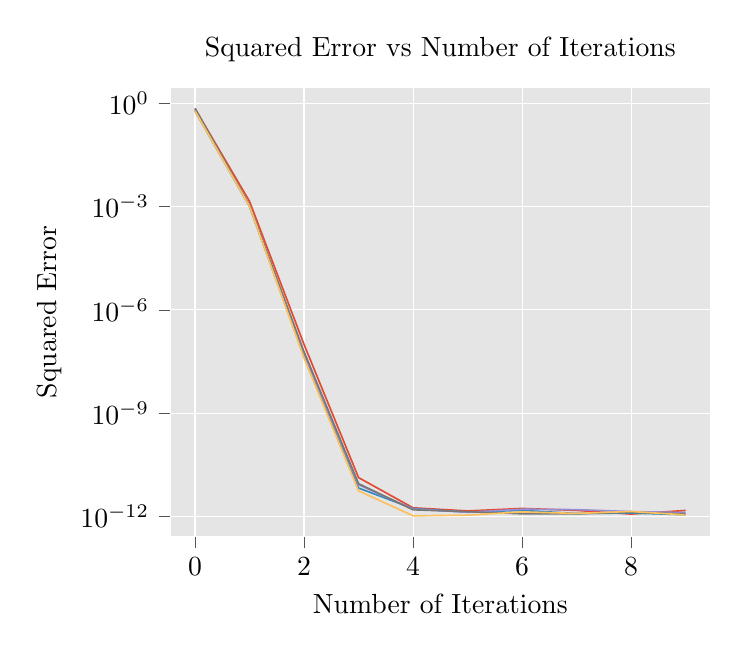
\begin{tikzpicture}

\definecolor{color0}{rgb}{0.886274509803922,0.290196078431373,0.2}
\definecolor{color1}{rgb}{0.203921568627451,0.541176470588235,0.741176470588235}
\definecolor{color2}{rgb}{0.596078431372549,0.556862745098039,0.835294117647059}
\definecolor{color3}{rgb}{0.984313725490196,0.756862745098039,0.368627450980392}

\begin{axis}[
axis background/.style={fill=white!89.8039215686275!black},
axis line style={white},
log basis y={10},
tick align=outside,
tick pos=left,
title={Squared Error vs Number of Iterations},
x grid style={white},
xlabel={Number of Iterations},
xlabel near ticks,
xmajorgrids,
xmin=-0.45, xmax=9.45,
xtick style={color=white!33.3333333333333!black},
y grid style={white},
ylabel={Squared Error},
ylabel near ticks,
ymajorgrids,
ymin=2.71273553797183e-13, ymax=2.77667975831396,
ymode=log,
ytick style={color=white!33.3333333333333!black}
]
\addplot [semithick, color0]
table {%
0 0.691431879997253
1 0.00141645281109959
2 9.95126896441434e-08
3 1.36033406761271e-11
4 1.80833126250945e-12
5 1.46727074934461e-12
6 1.73372427525464e-12
7 1.52411416820541e-12
8 1.19015908239817e-12
9 1.51345602716901e-12
};
\addplot [semithick, color1]
table {%
0 0.591166257858276
1 0.0010115496115759
2 4.45605756738132e-08
3 6.77857769915136e-12
4 1.71951342053944e-12
5 1.35713662530179e-12
6 1.52411416820541e-12
7 1.23634436022257e-12
8 1.27897692436818e-12
9 1.13686837721616e-12
};
\addplot [semithick, color2]
table {%
0 0.625002205371857
1 0.00102552131284028
2 5.11129663038901e-08
3 8.41993141875719e-12
4 1.66622271535743e-12
5 1.34292577058659e-12
6 1.64490643328463e-12
7 1.60227386913903e-12
8 1.406874616805e-12
9 1.31450406115619e-12
};
\addplot [semithick, white!46.6666666666667!black]
table {%
0 0.711470305919647
1 0.00108080555219203
2 6.08989694228512e-08
3 9.08784159037168e-12
4 1.58451030074502e-12
5 1.3962164757686e-12
6 1.21147536447097e-12
7 1.21147536447097e-12
8 1.33937305690779e-12
9 1.20792265079217e-12
};
\addplot [semithick, color3]
table {%
0 0.590315997600555
1 0.00102019123733044
2 3.97954451614169e-08
3 5.62394575354119e-12
4 1.05870867628255e-12
5 1.10844666778576e-12
6 1.37845290737459e-12
7 1.24344978758018e-12
8 1.4175327578414e-12
9 1.12265752250096e-12
};
\end{axis}

\end{tikzpicture}

        \caption{Demonstration of RAS convergence: 5 samples with $N=100$, randomly generated from a uniform distribution $[0,\frac{2}{N})$. Error is equal to the sum of squared errors of the sums of the rows and columns from 1. Note the logarithmic scale.}%
        \label{fig:ras_demo}
\end{figure}


\subsubsection{Non-negative Matrices}%
\label{ssub:non_negative_matrices}

Both because Sinkhorn-Knopp requires a non-negative matrix and because negative probabilities do not make sense, we have to ensure that the entries within $S$ are above  $0$. To do that, we can simply take the absolute value of all the entries, before applying RAS.
\begin{equation}
K'_{ij}=|K_{ij}|
\end{equation}

\subsection{Gradient Descent}%
\label{sub:gradient_descent}
Gradient Descent is an algorithm to iteratively optimize a convex function, with knowledge of the derivative of the function with respect to all of the function parameters $\theta$. In the case of optimizing a loss function, steps must be taken in the direction opposite to the gradient, therefore, the equation is as follows
\begin{equation}
         \theta'=\theta-\alpha \frac{\delta}{\delta \theta}L(\theta)
\end{equation}
where $\alpha$ is a parameter determining how big of a change there is between iterations of gradient descent.

\subsubsection{Negative Standard Deviation}%
\label{ssub:negative_standard_deviation}
In order to encourage discreteness, we can encourage sparseness within the matrix. That is, we would like one value to be larger than the others, this will help the algorithm within \ref{sec:discretization}. A common known metric to measure the spread of the data is called the standard deviation, and the biased standard deviation\footnote{Used for simplicity} is defined as follows:
\begin{align*}
    \frac{\sum_i^N \left(x_i-\overline{x}\right)^2}{N}
\end{align*}
But we want to have the value to increase when the spread decreases, so instead, we can the loss is the negative of the standard deviation. But we do not want to measure the spread against the mean, but rather, against the maximum (we want a single large maximum) so we take the negative of the maximum deviation:
\begin{align*}
    -\frac{N}{\sum_i^N \left(x_i-\max{x}\right)^2}
\end{align*}

\subsubsection{Derivative Coming Soon}%
\label{ssub:derivative_coming_soon}

\subsubsection{Partial Derivative of Loss Function}%
\label{ssub:derivative_of_loss_function}
The derivative of a multi-variable function \wrt{} a single variable, is called a partial-derivative, and is denoted by $\frac{\delta}{\delta x}$ instead of $\frac{d}{dx}$. Since our goal is to update each of the paramaters within $S$, we need to find a matrix which contains partial derivatives of the loss funtion against all of the elements.\footnote{This is very similar to Jacobian matrices; except that the Jacobian takes the partial derivatives of a vector against a vector, but we are taking partial derivatives of a scalar against a matrix.} That is, we are trying to find:
 \begin{align*}
         \frac{\delta L(S)}{\delta S}= \begin{bmatrix}
                 \frac{\delta L(S)}{\delta S_{1,1}}&\cdots &\frac{\delta L(S)}{\delta S_{1,N^2}}\\
                 \vdots &\ddots &\vdots \\
                 \frac{\delta L(S)}{\delta S_{N^2,1}}&\cdots &\frac{\delta L(S)}{\delta S_{N^2,N^2}}\\
         \end{bmatrix}
\end{align*}

To do that, we need to find the general solution to the partial derivative: $ \frac{\delta L(S)}{\delta S_{i,j}}$. Recall that the loss function is defined as
\begin{align*}
    L(S)=\frac{1}{2}\sum_{a}^{N^2} \sum_{b}^{N^2} \sum_{c}^{N^2} \sum_{d}^{N^2} S_{a,b} S_{c,d} C(O)_{a,c}C(O)_{b,d}
\end{align*}
Recall that in partial derivatives, only the variable in question (ie. $S_{i,j}$) is treated as a variable, the rest are treated as constants. We can see that the term $S_{i,j}$ is included within the loss when $(a,b)=(i,j)$ or $(c,d)=(i,j)$ or both. The derivatives are as following:
\begin{align*}
        \bm{A}=\frac{\delta L(S)}{\delta S_{i,j}}&=\frac{\delta}{\delta S_{i,j}}\left(\frac{1}{2}\sum_{c}^{N^2} \sum_{d}^{N^2} S_{i,j} S_{c,d} C(O)_{i,c}C(O)_{j,d}\right)&\text{First case}\\
              &=\frac{1}{2}\sum_{c}^{N^2} \sum_{d}^{N^2} S_{c,d} C(O)_{i,c}C(O)_{j,d}&\\
        \bm{B}=\frac{\delta L(S)}{\delta S_{i,j}}&=\frac{\delta}{\delta S_{i,j}}\left(\frac{1}{2}\sum_{a}^{N^2} \sum_{b}^{N^2} S_{a,b} S_{i,j} C(O)_{a,i}C(O)_{b,j}\right)&\text{Second case}\\
              &=\frac{1}{2}\sum_{a}^{N^2} \sum_{b}^{N^2} S_{a,b} C(O)_{a,i}C(O)_{b,j}&\\
        \bm{C}=\frac{\delta L(S)}{\delta S_{i,j}}&=\frac{\delta}{\delta S_{i,j}}\left(\frac{1}{2}S_{a,b} S_{a,b} C(O)_{a,b}C(O)_{a,b}\right)&\text{Third case}\\
              &=\frac{1}{2}\sum_{a}^{N^2} \sum_{b}^{N^2} S_{a,b} C(O)_{a,a}C(O)_{b,b}&\\
              &=0&
\end{align*}
$\bm{C}$ is $0$ because of the comparisons of tokens against themselves. The partial derivative of $L(S)$ against $S_{i,j}$ is equal to $\bm{A}+\bm{B}-\bm{C}=\bm{A}+\bm{B}$, because $\bm{A}$ and $\bm{B}$ represent all the cases in which $S_{i,j}$ is part of the loss function. Now, we can optimize $S$ with the Gradient Descent:
\begin{align*}
        S_{i,j}'=S_{i,j}-\alpha \left(\bm{A}+\bm{B}\right)
\end{align*}

\subsection{Optimization Procedure}%
\label{sub:optimization_procedure}

\subsubsection{Multi-objective Loss Function}%
\label{ssub:multi_objective_loss_function}
Now, we are satisfying multiple objectives: the negative maximum deviation, and the toroidal grid loss too. We can scale these by the losses by arbitrary parameters $\beta$ and $\gamma$

With all of the steps above, we can now optimize $S$. The procedure used within this essay is as following:\footnote{The procedure is by no means optimal. The purpose of this essay is not to be optimal, but to provide insight on what is possible.}
\begin{enumerate}
    \item Randomly initialize $S$ from a Uniform Distribution (equal probabilities for all values) on the interval $[0,1)$
    \item Repeat until convergence
    \begin{enumerate}
    \item Sum the Negative Maximum Deviation of all the rows and columns, and the Grid loss
    \item Calculate the partial derivatives
    item Perform Gradient Descent
    \end{enumerate}
\end{enumerate}

\section{Discretization}%
\label{sec:discretization}
Recall that our end goal is not to optimize the continuous representation of the toroidal grid, $S$, but rather the discrete grid $X$. To be able to convert $S$ into $X$, we must take into account the tokens in the positions with the highest confidence. And once this token is established within $X$, all of the entries within $S$ within the same token value (ie. same row), or same position (ie. same column) should be removed. This should be repeated until all the entries within $X$ are filled.

Let $r$ and $c$ (representing rows and columns) be empty sets. The procedure is then as following.
\begin{align*}
    r,c\leftarrow r,c\cup \argmax_{m\notin r,n\notin c}S_{m,n}\\
    X_{i,j}=O_{k,l}
\end{align*}
while $\argmax$ is defined. The conversion from $m$ and $n$ to $i,j$ and $k,l$ is stated within \ref{ssub:token_comparisons}.

\subsection{A Comprehensive Example}%
\label{sub:a_comprehensive_example}



\section{Evaluation}%
\label{sec:evaluation}
\subsection{Graphs of Loss over Time}%
\label{sub:graphs_of_loss_over_time}
\begin{figure}[htpb]
    \centering
    \includegraphics[width=0.8\linewidth]{images/invloss.png}
    \caption{Negative of Maximum Deviation vs Iterations}%
\end{figure}
\begin{figure}[htpb]
    \centering
    \includegraphics[width=0.8\linewidth]{images/gridloss.png}
    \caption{Superposition Loss vs Iterations}%
\end{figure}
\begin{figure}[htpb]
    \centering
    \includegraphics[width=0.8\linewidth]{images/real_loss.png}
    \caption{Discretized Grid Loss vs Iterations}%
\end{figure}

From the following images, we can see that Gradient Descent is in fact viable for Toroidal Grid Optimization \emph{in its continuous representation}, and that its success does not translate well over to the discretized version of the grid. This is reflected by the fact that the discretized loss after the optimization is worse off than it was in the beginning, during random initialization. This reflects a clear discrepancy between continuous and discrete optimization. The non-smoothness of 2 of the graphs can be traced to the non-discrete natures of both of those losses.

\subsection{Limitations}%
\label{sub:limitations}
A multi-objective loss function is difficult to optimize by nature. How much each component affects the overall loss function is to be determined arbitrarily, and these hyper-parameters\footnote{Parameters that cannot be learnt}, have to be tested arbitrarily. In this essay, only a single set of hyperparameters such as learning rate, proportion of negative maximum deviation and toroidal grid loss is used. This essay by no means provides a comprehensive evaluation of the possible optimization strategies, and therefore, may lack to optimize the function because of the wrong tuning of these hyperparameters and not a mistaken problem formulation.

The second possible reason is that I have not properly enforced the idea of discreteness within the optimization. There are a plentiful amount of methods to attempt this, including the Sinkhorn-Knopp algorithm for doubly stochastic matrices, and normal standard deviation. But through my trials, all of them work just about the same, which does not say a lot.

\subsection{Summary}%
\label{sub:summary}
Gradient descent is truly an amazing optimization algorithm. That is, if your loss function reflects the objective. But in the case of toroidal grid optimization, that does not seem to be the case. The stark difference between the continuous and the discrete nature of the problem of toroidal grid optimization makes gradient descent not a viable choice for this problem, according to the experiments laid out within this essay. But this does not hinder the effectiveness of Gradient Descent, but rather it highlights how it should be used properly. With a continuous objective.



\section{Acknowledgements}%
\label{sec:acknowledgements}

I would like to thank Emmerich Education Center for kindly providing computational resources used within this Extended Essay.


\printbibliography
\end{document}
